\chapter{\textgreek{Μεθοδολογία}}
\label{chapter_2}

\pagestyle{fancy}
\fancyhf{}
%\fancyhead[OC]{\leftmark \textgreek{Τι φάση}}
%\fancyhead[C]{}
%\fancyhead[EC]{\rightmark}
\renewcommand{\footrulewidth}{0.5pt}
\cfoot{\thepage}

\section{\textgreek{Εισαγωγή}}
\textgreek{Στο κεφάλαιο αυτό θα συζητήσουμε για τις μεθόδους και τις τεχνικές που χρησιμοποιήθηκαν στην εργασία μας αλλά και την ανάλυση με λεπτομέρειες των αλγορίθμων που εφαρμόστηκαν. Συγκεκριμένα, θα δούμε τις αρχιτεκτονικές βαθειάς μάθησης που χρησιμοποιήσαμε στα πειράματα, καθώς και την θεωρία αυτών. Η μεθοδολογία μας βασίστηκε στους αλγορίθμους των Νευρωνικών Δικτύων και πιο συγκεκριμένα στα Πλήρως Συνελικτικά Νευρωνικά Δίκτυα} FCNN \textgreek{που έχουν εφαρμογές σε προβλήματα της όρασης υπολογιστών και πιο συγκεκριμένα στην Σημασιολογική Κατάτμηση πληροφορίες από εικόνες. Η προσέγγιση μας περιλαμβάνει δύο μοντέλα τα οποία αποτελούνται από τρία στάδια: Κωδικοποίηση Χαρακτηριστικών, Παράλληλη Επεξεργασία και Αποκωδικοποίηση} (Encoder-Parallel Processing-Decoder). 

\section{\textgreek{Πρώτη Προσέγγιση}} 
\textgreek{Η πρώτη μας προσέγγιση στο πρόβλημα βασίστηκε σε μια παράλληλη αρχιτεκτονική από πολλαπλά ΣΝΔ (εικόνα} \ref{fig:cnn_1}). \textgreek{Η ιδέα στηρίχθηκε στην υλοποίηση τεσσάρων ΣΝΔ όπου τα 3 από αυτά δέχονται σαν είσοδο σειριακά κομμάτια από την εικόνα. Η μέθοδος αυτή αναφέρεται ως \emph{``Ολίσθηση Παραθύρων``}} \emph{(Sliding-Windows)} \cite{sliding_window}. \textgreek{Τα τρία από τα τέσσερα ΣΝΔ δέχονται κομμάτια διαφορετικού μεγέθους από την εικόνα, ενώ το τέταρτο ΣΝΔ δέχεται σαν είσοδο ολόκληρη την εικόνα. Έτσι παίρνουμε 4 διαφορετικές προβλέψεις για κάθε εικονοστοιχείο και αποφασίζουμε κατά πλειψηφία το επικρατέστερο.}\par

\textgreek{Η ιδέα αυτή αν και πολύ απλή είχε αρκετές δυσκολίες}:

\begin{description}[labelindent=10pt, style=multiline, leftmargin=30pt]
 \item[1.] \textgreek{Τα μικρά κομμάτια τμηματοποιούν κάποια αντικείμενα κατά την εκπαίδευση και καθίσταται δύσκολη η αναγνώριση τους καθώς δεν μαθαίνουν κάποια ολοκληρωμένη δομή από αυτά.}
 \item[2.] \textgreek{Η διαδικασία της δοκιμής ήταν σχεδόν ανέφικτη καθώς ένα τέτοιο μοντέλο είναι πολύ δαπανηρό σε πόρους.}
 \item[3.] \textgreek{Η μέθοδος Ολίσθησης Παραθύρων είναι πολύ αργή.}
\end{description}

\par \textgreek{Σύμφωνα με τα παραπάνω, δεν θα ασχοληθούμε περαιτέρω με αυτή την αρχιτεκτονική, αλλά προχωρήσαμε σε διαφορετική προσέγγιση του προβλήματος όπως θα δούμε στην συνέχεια.}

\begin{figure}[H]
 \centering
 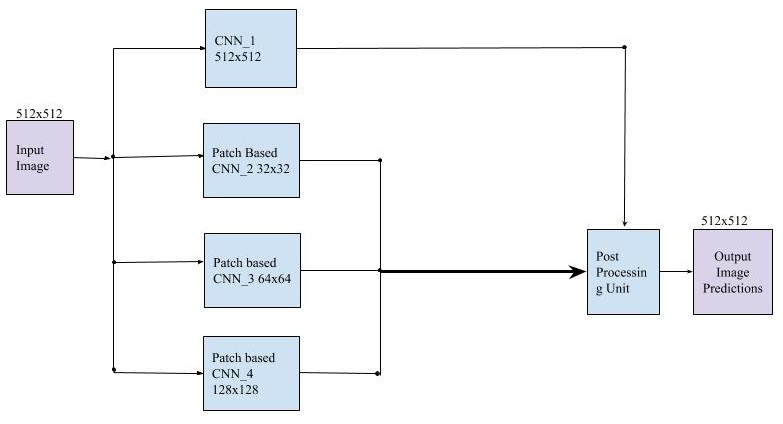
\includegraphics[scale=0.5]{Images/patch_cnn}
 \caption[\textgreek{Παράλληλο ΣΝΔ}]{\textgreek{Παράλληλη αρχιτεκτονική βασισμένη σε πολλαπλά ΣΝΔ με διαφορετικά μεγέθη ειδόδου το καθένα. }}
  \label{fig:cnn_1}
\end{figure}


\section{\textgreek{Προετοιμασία Δεδομένων}}
\textgreek{Η προετοιμασία των δεδομένων μας αποτελεί το πρώτο στάδιο, το οποίο κρίνεται αναγκαίο ώστε να γίνει εφικτή η εφαρμογή των αλγορίθμων βαθειάς μάθησης καθώς χωρίς αυτό το στάδιο δεν θα μπορέσουμε να έχουμε τα επιθυμητά αποτελέσματα.} 

\subsection{\textgreek{Υποδειγματοληψία}}
\label{sec:bilinear}
\textgreek{Η βάση δεδομένων μας αποτελείται από εικόνες υψηλής ευκρίνειας. Τα νευρωνικά δίκτυα έχουν πολλά εκατομμύρια παραμέτρους, οι παράμετροι είναι συνάρτηση της εισόδου του νευρωνικού δικτύου, επομένως η υποδειγματοληψία στις αρχικές εικόνες είναι απαραίτητη για να μπορέσουμε να κάνουμε εφικτά τα πειράματά μας. Αυτή η τεχνική φυσικά έχει κάποιο κόστος, καθώς η μείωση των διαστάσεων των εικόνων σημαίνει απώλεια σε πληροφορία. 


Για την υποδειγματοληψία στις εικόνες χρησιμοποιήθηκαν δύο διαφορετικοί αλγόριθμοι. Ο πρώτος είναι ο αλγόριθμος της Διγραμμικής Παρεμβολής} (Bilinear Interpolation) \textgreek{και ο δεύτερος είναι αυτός των Πλησιέστερων Γειτόνων.

\par 
Τον αλγόριθμο της Διγραμμικής Παρεμβολής τον χρησιμοποιήσαμε για την υποδειγματοληψία της εικόνας καθώς το εικονοστοιχείο που δημιουργείται κατά την διαδικασία της υποδειγματοληψίας προσεγγίζεται από μια σταθμισμένη εκτίμηση από άλλα τέσσερα σημεία ως μια καλύτερη προσέγγιση των εικονοστοιχείων.}


\textgreek{Ο αλγόριθμος του Πλησιέστερου Γείτονα, γνωστός και ως αλγόριθμος Παρεμβολής μηδενικής τάξης εφαρμόστηκε στις εικόνες με τις ετικέτες των εικονοστοιχείων} (ground truth). \textgreek{Ο λόγος που χρησιμοποιήσαμε αυτήν την απλή προσέγγιση είναι η εξασφάλιση των επιθυμητών ετικετών κατά τη διάρκεια της δειγματοληψίας. Συγκεκριμένα, το καινούριο εικονοστοχείο προέρχεται από το πλησιέστερο ως προς το μέγεθος εικονοστοιχείο, επομένως κάποιος άλλος αλγόριθμος θα μας παραποιούσε τις ετικέτες των εικονοστοιχείων. }

% \begin{figure}[h]
% %  \centering
% %  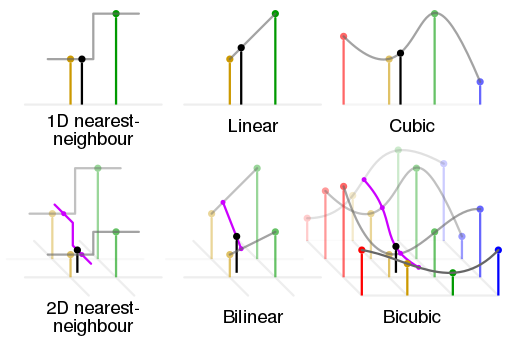
\includegraphics[scale=0.7]{Images/all_inter}
% %  \caption[\textgreek{Μέθοδοι Παρεμβολής}]{\textgreek{Μέθοδοι Παρεμβολής} \cite{wiki_interpolation}.}
%  \label{fig:all_inter_img}
% \end{figure}

\subsection{\textgreek{Κανονικοποίηση Χαρακτηριστικών}}
\textgreek{Η  κανονικοποίηση των χαρακτηριστικών }(feature normalization),\textgreek{ εφαρμόζεται στα χαρακτηριστικά των δεδομένων, στην δική μας περίπτωση τις εικόνες και έχει ως αποτέλεσμα να φέρει τα δεδομένα στην ίδια κλίμακα με μικρές διακυμάνσεις μεταξύ τους. Ο χώρος των χρωμάτων των εικόνων έχει μεγάλο εύρος $[0,255]$. Αυτό δημιουργεί πρόβλημα στην εκπαίδευση των ΝΔ καθώς μπορεί να πάρουν ανεξέλεγκτες τιμές οι νευρώνες στα }hidden layers \textgreek{και να μην συγκλίνει το ΣNΔ Ο λόγος που βελτιώνει την σύγκλιση είναι επειδή οι τιμές στην είσοδο έχουν μέση τιμή μηδέν και διασπορά ένα, ως αποτέλεσμα οι νευρώνες στα ενδιάμεσα επίπεδα δεν μπαίνουν σε κορεσμό τόσο εύκολα και τόσο γρήγορα. Η εξίσωση }\ref{eqn:eq_feat_norm} \textgreek{μας εξασφαλίζει τα χαρακτηριστικά να βρίσκονται στον χώρο $[-1,1]$, έχοντας μέση τιμή μηδέν και διασπορά κοντά στο ένα. Για τον υπολογισμό της μέσης τιμής του συνόλου δεδομένων χρησιμοποιήσαμε ένα δείγμα από αυτό, από 500 δείγματα} \cite{feat_norm}.


\begin{equation}
 \hat{\mu} = \frac{\sum_{i=1}^{N} X_{i}}{N} 
 \label{mean}
\end{equation}
\\[1cm]

\begin{equation}
 X = \frac{X - \hat{\mu}}{max(X) - min(X)}
 \label{eqn:eq_feat_norm}
\end{equation}

\subsection{\textgreek{Δυσαναλογία των Κλάσεων}}
\textgreek{Ένα πολύ συχνό πρόβλημα που υπάρχει στα περισσότερα σύνολα δεδομένων, είναι η δυσαναλογία των κλάσεων ή κατηγοριών. Η δυσαναλογία προκύπτει όταν σε ένα σύνολο δεδομένων υπάρχουν μεγάλες διαφορές μεταξύ του πλήθους των στοιχείων που ανήκουν σε ορισμένες κατηγορίες. Το πρόβλημα αυτό δεν το λύνουν τα νευρωνικά δίκτυα από μόνα τους, καθώς τείνουν να μάθουν καλύτερα πληροφορίες για τα στοιχεία που αποτελούν πλειοψηφία στο σύνολο δεδομένων μας, ενώ τα στοιχεία που αποτελούν μειονότητα φτάνουν σε σημείο μέχρι και να αγνοούνται. Μία λύση σε αυτό το πρόβλημα θα μπορούσε να είναι η υπερδειγματοληψία των κλάσεων που είναι μειονότητα, έτσι ώστε να δημιουργήσουμε ισόποσα σύνολα κλάσεων για να υπάρξει ισοστάθμιση. Όμως αυτή η τεχνική είναι ανέφικτη σε ένα σύνολο από εικόνες όπου θα πρέπει να δημιουργήσουμε καινούρια εικονοστοιχεία που να ανήκουν σε κάποια συγκεκριμένη κατηγορία. 

\par Για την λύση αυτού του προβλήματος εφαρμόστηκε η Συνάρτηση Μέσης Συχνότητας Ισορροπίας }(Median Frequency Balance) \cite{median_freq}. \textgreek{Με αυτή την συνάρτηση βρίσκουμε τους συντελεστές και τους εφαρμόζουμε στην συνάρτηση κόστους (εξίσωση} \ref{eqn:loss_func}). \textgreek{\par Η ιδέα είναι να βρεθούν οι συντελεστές συχνότητας οι οποίοι προέρχονται από την συχνότητα εμφάνισης ενός εικονοστοιχείου που ανήκει σε μια κατηγορία. Όταν ένα εικονοστοιχείο $i$ ανήκει στην κατηγορία $j$ (όπου είναι μειονότητα) και βρίσκεται κατά την διαδικασία της μάθησης να είναι στην κατηγορία $k$ τότε επιβάλλεται μεγαλύτερη ποινή και διαδίδεται μεγαλύτερο σφάλμα προς τα πίσω. Αυτό συμβαίνει επειδή το νευρωνικό δίκτυο δεν θα δει πολλές φορές μια κλάση που είναι μειονότητα οφείλουμε να εισάγουμε μεγαλύτερη ποινή για να βοηθήσουμε στην εκμάθηση τους. 

\par Με την εξίσωση }\ref{eqn:ratio} \textgreek{βρίσκουμε την συχνότητα εμφάνισης των εικονοστοιχείων για κάθε κλάση στο σύνολο δεδομένων και αφού ταξινομήσουμε τις τιμές συχνότητας παίρνουμε την μεσαία συχνότητα και την χρησιμοποιούμε σαν επίκεντρο} \textgreek{τοποθετώντας την στον αριθμητή (εξίσωση }\ref{eqn:alpha_coef}). \textgreek{Με αυτή την μέθοδο πετυχαίνουμε να έχουμε υψηλούς συντελεστές $a_i$ στα χαμηλής συχνότητας εμφάνισης εικονοστοιχεία. Με την εξίσωση} \ref{eqn:alpha_coef} \textgreek{βρίσκουμε τους συντελεστές $a$ για κάθε κατηγορία αντικειμένων. Ένας μεγάλος συντελεστής $a_i$ προσθέτει μεγαλύτερη ποινή όταν ταξινομηθεί λάθος ένα εικονοστοιχείο που ανήκει σε μια κλάση που δεν υπάρχει πολλές φορές στο σύνολο δεδομένων. Τέλος, στα δεδομένα μας, υπάρχουν εικονοστοιχεία τα οποία δεν ανήκουν σε κάποια κατηγορία, για να μην μάθει το ΝΔ από αυτά θέσαμε τον συντελεστή $a_i$ στο μηδέν έτσι ώστε να μην συνεισφέρουν στο σφάλμα κατά την εκπαίδευση.} 

\noindent\begin{minipage}{.5\linewidth}
  \begin{equation}
    freq(C_{i}) = \frac{C_{i}}{\sum_{i=1}^{Classes} C_{i}}
    \label{eqn:ratio}
  \end{equation}
\end{minipage}%
\begin{minipage}{.5\linewidth}
  \begin{equation}
  \alpha_{i} = \frac{median(freq)}{freq(C_{i})}
  \label{eqn:alpha_coef}
  \end{equation}
\end{minipage}


\subsection{\textgreek{Επισκόπηση Αρχιτεκτονικής}}

\subsubsection{\textgreek{Αρχικοποίηση Παραμέτρων Πυρήνα}}
\textgreek{Η αρχικοποίηση των παραμέτρων των φίλτρων αποτελεί ένα σημαντικό στάδιο στην εκπαίδευση των Νευρωνικών Δικτύων. Στόχος της αρχικοποίησης είναι η μέση τιμή της εισόδου και εξόδου ενός επιπέδου να είναι κοντά στο μηδέν αλλά και η διασπορά τους να είναι κοντά στο ένα, καθώς αποτρέπει τους Νευρώνες να μπουν σε κορεσμό. Τα βάρη του ΣΝΔ δειγματοληπτήθηκαν από μία Γκαουσιανή κατανομή με μέση τιμή ίση με το μηδέν ($\mu=0$) και διασπορά ίση με ένα ($\sigma^2 = 1/N$). Η εξίσωση} \ref{eqn:lecun_norm} \textgreek{μας δείχνει την τυπική απόκλιση που εφαρμόστηκε στην κατανομή Γκάους (εξίσωση} \ref{eqn:gauss}) \textgreek{για την δειγματοληψία των βαρών όπου με $N$ συμβολίζεται το πλήθος των χαρακτηριστικών της εισόδου σε κάθε επίπεδο συνέλιξης. } 

\begin{equation}
 \label{eqn:lecun_norm}
  \centering
 \mathit{\sigma} = \sqrt{\frac{1}{\textit{N}}}
\end{equation}

\begin{equation}
 \label{eqn:gauss}
  \centering
 g(x) = \frac{1}{\sigma \sqrt{2\pi}} e^{\frac{1}{2}(\frac{x-\mu}{\sigma})^{2}}
\end{equation}

\subsubsection{\textgreek{Συνάρτηση Ενεργοποίησης}}
\textgreek{Άλλη μια απαραίτητη συνάρτηση για τα Νευρωνικά Δίκτυα είναι η συνάρτηση ενεργοποίησης. Εφαρμόζεται στην έξοδο των επιπέδων των νευρωνικών δικτύων και είναι υπεύθυνη για την ανταλλαγή μηνυμάτων μεταξύ νευρώνων στα επίπεδα από νευρώνες. Τα βαθειά νευρωνικά δίκτυα έρχονται αντιμέτωπα με το πρόβλημα της εξαφάνισης των αποκλίσεων του σφάλματος κατά την διάδοσή τους προς τα πίσω. Για τον λόγο αυτό επινοήθηκαν συναρτήσεις που ονομάζονται Γραμμικοί Ανορθωτές }(Linear Rectifiers). \textgreek{Οι γραμμικοί ανορθωτές συνήθως κάτω από το μηδέν έχουν μηδενική τιμή. Όταν οι αποκλίσεις πέφτουν κάτω από το μηδέν τα βάρη δεν αλλάζουν, δηλαδή οι νευρώνες μένουν απενεργοποιημένοι σε μια τέτοια περίπτωση. Το θετικό σε αυτήν την περίπτωση είναι ότι εφόσον κάποιοι νευρώνες τείνουν σε αδράνεια, το νευρωνικό γίνεται ελαφρύτερο από την άποψη των υπολογισμών. Από την άλλη, το μεγάλο μειονέκτημα είναι ότι αν βρεθούν σε αυτή την κατάσταση μπορεί να μην ξανά ενεργοποιηθούν οι νευρώνες και δεν θα ανταποκριθούν σε αλλαγές από μικρά σφάλματα. Αυτό ονομάζεται Φαινόμενο Νεκρών Νευρώνων. 
\par Μία λύση σε αυτό το πρόβλημα είναι η εισαγωγή μιας παραμετρικής συνάρτησης κάτω από το μηδέν, η οποία θα δίνει ένα μικρό ερέθισμα στους νευρώνες ώστε να αποφευχθεί αυτό το πρόβλημα. Για τον λόγο αυτό εισάγαμε στα νευρωνικά μας την Κλιμακωτή Εκθετική Γραμμική Συνάρτηση }(Scaled Exponential Linear Unit-SELU). \textgreek{Στην πραγματικότητα όπως απέδειξαν στο }\cite{self_norm}\textgreek{ η συγκεκριμένη συνάρτηση ενεργοποίησης σε συνδυασμό με την αρχικοποίηση (εξισώσεις }\ref{eqn:lecun_norm}, \ref{eqn:gauss}) \textgreek{όχι μόνο καταπολεμά αυτό το πρόβλημα αλλά καθιστά περιττή την εφαρμογή του αλγορίθμου }Batch-Normalization \cite{batch_norm} \textgreek{καθώς η κανονικοποίηση των εισόδων σε κάθε επίπεδο του νευρωνικού γίνεται μέσα σε αυτή την συνάρτηση, πετυχαίνοντας έτσι μείωση των παραμέτρων.}

\begin{figure}[H]
 \centering
 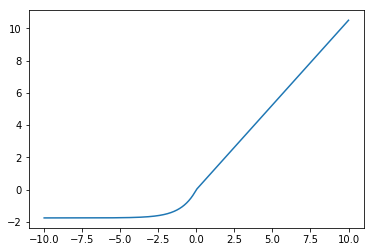
\includegraphics[scale=1.1]{Images/selu}
 \caption[SELU Function]{\textgreek{Κλιμακωτή Εκθετική Γραμμική Συνάρτηση Ενεργοποίησης} (SELU) \textgreek{με τις προεπιλεγμένες παραμέτρους $\alpha = 1.6732$\textgreek{ και} $\lambda = 1.0507$}.}
  \label{fig:selu_img}
\end{figure}


\begin{equation}
 f(x) = \lambda
\begin{cases}
    x   & \quad \text{if } x > 0 \\
    \alpha e^{x} - \alpha & \quad \text{if } x \leq 0
\end{cases}
\end{equation}


\begin{figure}[H]
 \label{act_func_img}
 \centering
 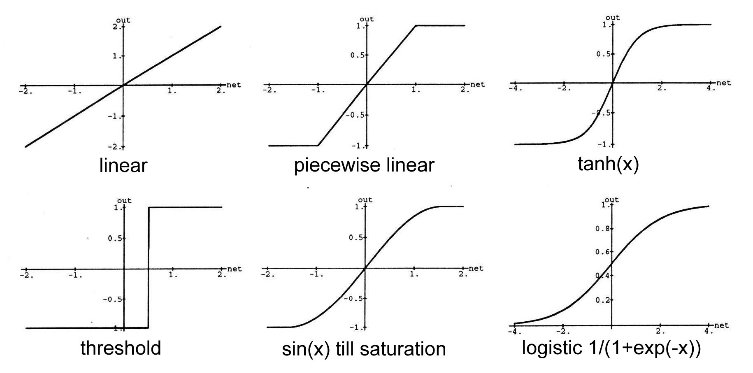
\includegraphics[scale=0.6]{Images/act_func}
 \caption[\textgreek{Συναρτήσεις Ενεργοποίησης}]{\textgreek{Διάφορες συναρτήσεις Ενεργοποίησης} \cite{act_funcs}}
\end{figure}


\subsubsection{\textgreek{Αλγόριθμοι Βελτιστοποίησης}}
\textgreek{Ο αλγόριθμος βελτιστοποίησης αποτελεί έναν πολύ σημαντικό παράγοντα για την εκπαίδευση ενός Νευρωνικού Δικτύου. Η ανάγκη για αναζήτηση αλγορίθμων βελτιστοποίησης προήλθε από δύο σημαντικούς παράγοντες. Πρώτον, λόγω των πολλών δεδομένων για επεξεργασία και των βαθιών νευρωνικών δικτύων που έκανε την διαδικασία της μάθησης αργή. Αυτοί οι λόγοι μας ώθησαν σε τεχνικές μείωσης του σφάλματος από κομμάτια του συνόλου δεδομένων και δεύτερων για την επιτάχυνση της σύγκλισης του Νευρωνικού δικτύου προφανώς.} 

\textgreek{Παρακάτω στην εικόνα }\ref{fig:sgd_regime} \textgreek{βλέπουμε πως αν η συνάρτηση κόστους έχει την μορφή μίας χαράδρας που οδηγεί προς το βέλτιστο κόστος και έχει στα πλάγια υψηλά τοιχώματα, τότε με ένα μεγάλο ρυθμό μάθησης τα βάρη τείνουν να ταλαντεύονται μπρος και πίσω επειδή η αρνητική απόκλιση τείνει προς τις απότομες πλευρές κάθε φορά αντί να πηγαίνει προς το βέλτιστο. Αυτό το φαινόμενο συμβαίνει σχεδόν πάντα και δημιουργεί πρόβλημα διότι μας κάνει την σύγκλιση πολύ αργή.}

\begin{figure}[H]
 \centering
 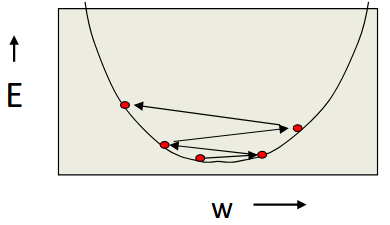
\includegraphics[scale=0.5]{Images/sgd_img}
 \caption[\textgreek{Ενέργεια Συνάρτησης Κόστους}]{\textgreek{Ταλάντωση κατά την εκτίμηση των βαρών όπου ο μεγάλος ρυθμός μάθησης οδηγεί σε αντίθετο αποτέλεσμα} \cite{coursera_nn}.}
 \label{fig:sgd_regime}
\end{figure}


\textgreek{Ο πιο συνηθισμένος και βασικός αλγόριθμος βελτιστοποίησης είναι ο Στοχαστικός Αλγόριθμος Απότομης καθόδου} (SGD) \cite{sgd}, \textgreek{ο οποίος υπολογίζει απλά την απόκλιση των παραμέτρων ως προς της συνάρτηση κόστους πάνω σε ένα μικρό σύνολο δειγμάτων από τα δεδομένα. Πλέον υπάρχουν πιο προχωρημένοι αλγόριθμοι βελτιστοποίησης που χρησιμοποιούν περισσότερες παραμέτρους. Η επιλογή του αλγόριθμου βελτιστοποίησης γίνεται ανάλογα με την αρχιτεκτονική του Νευρωνικού Δικτύου. Η εξίσωση} \ref{eqn:sgd_equation} \textgreek{μας δείχνει την εξίσωση όπου $\alpha$ είναι ο ρυθμός μάθησης και ο υπολογισμός της απόκλισης γίνεται πάνω σε ένα σύνολο ζευγών} $(x^{i},y^{j})$.
 

\begin{equation}
\label{eqn:sgd_equation}
 \vartheta = \vartheta - \alpha \nabla_{\vartheta}\mathit{\mathcal{J}(\vartheta;x^{i},y^{j})}
\end{equation}\\


\textgreek{Με την χρήση της παραμέτρους της ορμής, ο αλγόριθμος τείνει να φτάσει στο βέλτιστο σημείο πιο γρήγορα. Στην εξίσωση }\ref{eqn:sgd_eq_momentum} $\upsilon$ \textgreek{είναι το διάνυσμα ταχύτητας το οποίο είναι φυσικά ίδιων διαστάσεων με το διάνυσμα των παραμέτρων }$\theta$. \textgreek{Πέρα από την παράμετρο }$\alpha$ \textgreek{που είδαμε και προηγουμένως η οποία είναι ο ρυθμός μάθησης, παρατηρούμε και την παράμετρο }$\gamma \in [0,1)$ \textgreek{η οποία ορίζει το ποσοστό συνεισφοράς των προηγούμενων αποκλίσεων στην παρούσα ανανέωση των παραμέτρων. Συνήθως αυτή η ποσότητα ορίζεται στο $0.9$.} 

\begin{equation}   
 \label{eqn:sgd_eq_momentum}
 \begin{split}
     \upsilon &= \gamma \upsilon + \alpha \nabla_{\vartheta}\mathit{\mathcal{J}(\vartheta;x^{i},y^{j})}\\
     \vartheta &= \vartheta - \upsilon
 \end{split}
\end{equation}\\

\textgreek{Στην εργασία μας έγινε χρήση τόσο του αλγορίθμου της Στοχαστικής Απότομης Καθόδου, αλλά και του αλγόριθμου} Adam \cite{adam} \textgreek{ενός πιο αποδοτικού αλγορίθμου σε θέματα στοχαστικής βελτιστοποίησης καθώς χρησιμοποιεί πρώτης τάξης παραγώγους. Ο αλγόριθμος υπολογίζει τις παραμέτρους του ρυθμού μάθησης για διάφορες παραμέτρους από εκτιμήσεις των ορμών πρώτης και δεύτερης τάξης των κλίσεων, όπως φαίνεται αναλυτικά παρακάτω. }\textgreek{Συγκεκριμένα ο αλγόριθμος }Adam \textgreek{είναι μια εξέλιξη του} RMSProp \cite{rmsProp, DBLP:journals/corr/Ruder16}. 

\begin{algorithm}[H]
    \caption[\textgreek{Αλγόριθμος }Adam]{\textgreek{Αλγόριθμος} Adam \cite{DBLP:journals/corr/KingmaB14}. \textgreek{Αναλυτική περιγραφή των βημάτων, όλες οι πράξεις των διανυσμάτων είναι ανά στοιχείο. Η $g_{t}^{2}$ δείχνει τον ανά στοιχείο πολλαπλασιασμό $g_{t}\odot g_{t}$. Οι προτεινόμενες τιμές των παραμέτρων είναι: $\alpha = 0.001, \beta_{1}=0.9, \beta_{2}=0.999$ και $\epsilon=10^{-8}$}.}\label{alg:Algo_adam}
  \begin{algorithmic}[1]
    \REQUIRE $:\alpha:$ \textgreek{Ρυθμός Μάθησης} 
    \REQUIRE $\beta_{1},\beta_2 \in [0,1):$ \textgreek{Εκθετικοί ρυθμοί καθόδου για τις εκτιμήσεις των ορμών}
    \REQUIRE $f(\theta):$ \textgreek{Στοχαστική συνάρτηση κόστους}
    \REQUIRE $\theta_{0}:$ \textgreek{Αρχικοποίηση διανύσματος παραμέτρων}\\
    $m_{0} \gets 0:$ \textgreek{Αρχικοποίηση 1ης τάξης διανύσματος} \\
    $u_{0} \gets 0:$ \textgreek{Αρχικοποίηση 2ης τάξης διανύσματος} \\ 
    $t \gets 0:$ \textgreek{Αρχικοποίηση βήματος χρόνου}
    %\STATE \textbf{Initialization} ‎$R^{(0)} = x$
    \WHILE{$\theta_{t}$  \textit{ not converged } }
     \STATE $t = t + 1$\\
     
     \STATE{$g_{t} \gets \nabla_{\theta}f_{t}(\theta_{t-1})$} \COMMENT{\textgreek{Αποκλίσεις ως προς την συνάρτηση }f \textgreek{την στιγμή }t}\\
     
     \STATE $m_{t} \gets \beta_{1} \cdot m_{t-1} + (1 - \beta_{1}) \cdot g_{t}$ \COMMENT{\textgreek{Ενημέρωση της μεροληπτικής εκτίμησης 1ης τάξης}}\\
     
     \STATE $\upsilon_{t} \gets \beta_{1} \cdot m_{t-1} + (1 - \beta_{2}) \cdot g_{t}^{2}$ \COMMENT{\textgreek{Ενημέρωση της μεροληπτικής εκτίμησης 2ης τάξης}}\\
     \STATE $\hat{m}_{t} \gets m_{t}/(1 - \beta_{1}^{t})$ \COMMENT{\textgreek{Διόρθωση της μεροληπτικής εκτίμησης 1ης τάξης}}\\
     
     \STATE $\hat{\upsilon_{t}} \gets \upsilon_{t}/(1 - \beta_{2}^{t})$ \COMMENT{\textgreek{Διόρθωση της μεροληπτικής εκτίμησης 2ης τάξης}} \\
     
     \STATE $\theta_{t} \gets \theta_{t-1} - \alpha \cdot \hat{m_{t}}/(\sqrt{\hat{\upsilon_{t}}} + \epsilon) $ \COMMENT{\textgreek{Ενημέρωση παραμέτρων}}
           
    \ENDWHILE
    \RETURN $\theta_{t}$ \COMMENT{\textgreek{Αποτελέσματα παραμέτρων}}

  \end{algorithmic}
\end{algorithm}



\subsubsection{\textgreek{Συνάρτηση Κόστους}}
\label{sec:loss_function}
\textgreek{Συνήθως, σε προβλήματα πολλαπλής ταξινόμησης στοιχείων, όπως στην Σημασιολογική Κατάτμηση, θέλουμε τα Νευρωνικά Δίκτυα να δέχονται στην είσοδο ένα διάνυσμα και να μας δίνουν στην έξοδο ένα διάνυσμα με την πιθανότητα των εικονοστοιχείων να ανήκουν σε μια από τις $L$ κατηγορίες. Για να το επιτύχουμε αυτό τοποθετούμε ένα επίπεδο }\emph{Softmax $L$ }\textgreek{εξόδων, στην έξοδο του Νευρωνικού Δικτύου. Η }$softmax(z)_{i}$ \textgreek{περιγράφει την }$i_{th}$ \textgreek{πιθανότητα ενός εικονοστοιχείου να ανήκει σε μια από τις $L$ κατηγορίες. Η } \emph{softmax} \textgreek{μετατρέπει το διάνυσμα $L$ διαστάσεων σε μια πιθανοτική κατανομή όπου όλες οι τιμές αθροίζονται στο ένα (εξίσωση }\ref{eqn:softmax}).

\begin{equation}
  \label{eqn:softmax}
  \mathit{softmax(z)_{i}} = \frac{e^{z_{i}}}{\sum_{l=1}^{L} e^{z_{l}}}
\end{equation}
%\\[1cm]

\textgreek{Επειδή η έξοδος του ΝΔ είναι μια μονάδα }softmax, \textgreek{πρέπει να χρησιμοποιηθεί και η κατάλληλη συνάρτηση κόστους. Η συνάρτηση κόστους μετράει την διαφορά μεταξύ της εξόδου του ΝΔ και της επιθυμητής εξόδου. Όταν η έξοδος του ΝΔ είναι μια πιθανοτική κατανομή, η πιο κατάλληλη συνάρτηση κόστους είναι η αρνητική λογαριθμική πιθανότητα της επιθυμητής εξόδου. Η συνάρτηση αυτή ονομάζεται Συνάρτηση Διεντροπίας }(Cross-Entropy). \textgreek{Βέβαια λόγω της εισαγωγής των συντελεστών $\alpha$ στην συνάρτηση για την ισοστάθμιση των κλάσεων έχουμε παραμετροποιήσει την συνάρτηση καταλλήλως (εξίσωση }\ref{eqn:loss_func}). \textgreek{Με $p_{ij}$ συμβολίζεται η κατανομή των πραγματικών τιμών του εικονοστοιχείου $i$ που ανήκει σε μια κατηγορία $j$ ενώ με $q_{ij}$ συμβολίζεται η έξοδος που δίνει το μοντέλο για το εικονοστοιχείο $i$ με μια πιθανοτική κατανομή πάνω στις $L$ κατηγορίες του μοντέλου όπου $j\in L$. Στην πραγματικότητα, οι πραγματικές τιμές $p_{i}$ ενός εικονοστοιχείου είναι ένα διάνυσμα $L$ διαστάσεων όπου η σωστή κατηγορία που ανήκει το εικονοστοιχείο $i$ διαθέτει ένα στην θέση $j$ της σωστής κατηγορίας ενώ στις υπόλοιπες θέσεις των λάθος κατηγοριών διαθέτει μηδέν. Επίσης, έχουμε προσθέσει τους συντελεστές $\alpha_j$ οι οποίοι ρυθμίζουν την ποινή για κάθε λάθος πρόβλεψη κατηγορίας. Στο τέλος γίνεται μια κανονικοποίηση ως προς το πλήθος των εικονοστοιχείων της εικόνας $N$.}

\begin{equation}
\label{eqn:loss_func}
 \mathit{Loss} = - \frac{1}{N} \sum_{i\in N} \sum_{j\in L} p_{ij} log(q_{ij}) \alpha_{j}
\end{equation}

\textgreek{Κατά την εκπαίδευση ενός ΝΔ, αυτό που γίνεται είναι η βελτιστοποίηση της συνάρτησης κόστους }(cross-entropy). \textgreek{Με αυτό τον τρόπο χρησιμοποιούμε το σφάλμα από την συνάρτηση κόστους και επαναληπτικά επαναπροσδιορίζουμε τις παραμέτρους του ΝΔ με σκοπό να ελαχιστοποιήσουμε το κόστος. Η μείωση της συνάρτησης κόστους είναι ισοδύναμο με το γεγονός της αύξησης της πιθανότητας της σωστής απάντησης. }

\subsection{\textgreek{Στάδιο Κωδικοποίησης}}
\textgreek{Σκοπός της μονάδας Κωδικοποίησης είναι η εξαγωγή χαρακτηριστικών από την έγχρωμη εικόνα, δηλαδή η δημιουργία μιας αναπαράστασης πολυδιάστατων χαρακτηριστικών από τα εικονοστοιχεία της εικόνας σε μια συμπιεσμένη μορφή ώστε να γίνεται εφικτή η εκπαίδευση του συστήματος. Η μονάδα κωδικοποίησης αποτελείται από 4 τμήματα και συγκεκριμένα από ομάδες συνελικτικών επιπέδων και μονάδων συγκέντρωσης. Η εικόνα }\ref{fig:conv_block} \textgreek{μας δίνει μια διαίσθηση του κάθε τμήματος το οποίο αποτελείται από 2 επίπεδα συνέλιξης ακολουθούμενα από ένα επίπεδο συγκέντρωσης μέγιστων τιμών ανά περιοχή }(Max-Pooling). 


\begin{figure}[H]
 \centering
 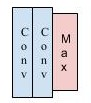
\includegraphics[scale=0.6]{Images/conv_block}
  \caption[\textgreek{Τμήμα Συνέλιξης}]{\textgreek{Τμήμα συνέλιξης: 2 επίπεδα συνέλιξης και ενα }Max-pooling \textgreek{επίπεδο.}}
 \label{fig:conv_block}
\end{figure}

\textgreek{Πιο συγκεκριμένα, στα επίπεδα συνέλιξης γεμίζουμε περιφερειακά την χαρτογράφηση των χαρακτηριστικών με μηδενικά ανάλογα με το μέγεθος του πυρήνα για να μπορέσουμε να κρατήσουμε το μέγεθος τους αναλλοίωτο κρατώντας την θέση των χαρακτηριστικών αλλά και επειδή χρειαζόμαστε την πληροφορία από τις γωνίες των χαρακτηριστικών. Η εικόνα }\ref{fig:conv_pad} \textgreek{μας δείχνει ένα παράδειγμα της διαδικασίας, ενώ η εξίσωση }\ref{eqn:half_pad} \textgreek{μας δείχνει ότι για να πετύχουμε μέγεθος εισόδου }(input) \textgreek{ίδιο με το μέγεθος εξόδου, πρέπει να ισχύει η παρακάτω εξίσωση, για οποιοδήποτε μέγεθος εισόδου }input \textgreek{και για μονό αριθμό στοιχείων πυρήνα $k$ όπου }($k = 2n + 1, n \in  \mathbb{N})$  \textgreek{, $s$ είναι το βήμα ολίσθησης το οποίο είναι 1 και δεν λαμβάνεται υπόψη στην εξίσωση. Με το }$p$ \textgreek{συμβολίζεται το γέμισμα των μηδενικών περιφερειακά της εισόδου όπου }$p = \lfloor k/2 \rfloor = n$.

\begin{equation}
\label{eqn:half_pad}
\begin{align*}
output &= input + 2\lfloor k/2 \rfloor -(k - 1) \\
        &= input + 2n - 2n \\
        &= input
\end{align*}
\end{equation}

\begin{figure}[H]
 \centering
 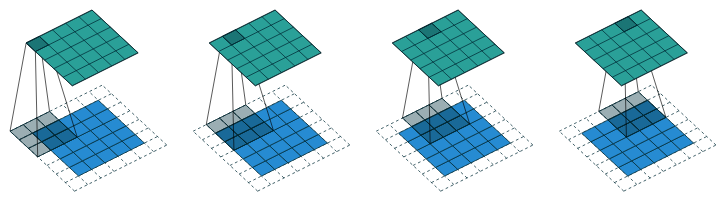
\includegraphics[scale=0.4]{Images/conv_pad}
  \caption[\textgreek{Συνέλιξη με }Zero-Padding]{\textgreek{Εφαρμογή ενός πυρήνα $3\times3$ με ολίσθηση μονού βηματισμού σε επίπεδο εισόδου μεγέθους $5\times5$ με γέμισμα μηδενικών περιφερειακά της εισόδου} \cite{conv_arithmetic}.}
 \label{fig:conv_pad}
\end{figure}


\textgreek{Το στάδιο κωδικοποίησης αποτελείται από 4 τμήματα (εικόνα }\ref{fig:conv_block})\textgreek{ όπου δέχεται σαν είσοδο την εικόνα μεγέθους $512\times512\times3$ και παράγει στην έξοδο μια χαρτογράφηση χαρακτηριστικών $32\times32\times256$, όπου η τρίτη διάσταση είναι ο αριθμός των φίλτρων. Πιο αναλυτικά στο πρώτο τμήμα έχουμε την συνέλιξη της εικόνας με μια σειρά από 32 φίλτρα και ακόμα ένα ίδιο επίπεδο πριν καταλήξουμε να εφαρμόσουμε το επίπεδο μέγιστης συγκέντρωσης. Το επίπεδο μέγιστης συγκέντρωσης είναι μια ανορθόδοξη τεχνική στην οποία επιδιώκουμε να μειώσουμε τον αριθμό των παραμέτρων σταδιακά, καθώς όσο προχωράμε στα επόμενα τμήματα αυξάνεται ο αριθμός του βάθους των επιπέδων (δηλαδή των φίλτρων) και επομένως και ο αριθμός των παραμέτρων. Ένας άλλος λόγος είναι η προσπάθεια της εξάλειψης της υπερμάθησης ως αποτέλεσμα της μείωσης των παραμέτρων. Στην δική μας περίπτωση συγκεντρώσαμε από κάθε περιοχή $2\times2$ την μέγιστη τιμή των χαρακτηριστικών. Συγκεκριμένα ολισθαίνουμε ένα παράθυρο μεγέθους $2\times2$ στα χαρακτηριστικά και παίρνουμε την μέγιστη τιμή. Διαισθητικά, αυτό σημαίνει ότι κρατήσαμε την τιμή που υπάρχει μεγαλύτερο ερέθισμα στον εκάστοτε νευρώνα (εικόνα }\ref{fig:maxpool}). \textgreek{Επομένως ο χάρτης των χαρακτηριστικών χώρου μετά από κάθε τμήμα μειώνεται κατά το ήμισυ, οι εξισώσεις παρακάτω μας δείχνουν τον υπολογισμό των διαστάσεων εξόδου μετά την εφαρμογή του επιπέδου μέγιστης συγκέντρωσης. Η μεταβλητή $P$ ορίζει τυχόν γέμισμα στο στάδιο της συγκέντρωσης το οποίο στην δική μας περίπτωση είναι μηδέν και με $S$ ορίζεται το άλμα ολίσθησης του πυρήνα συγκέντρωσης το οποίο είναι ίσο με 2.} 


\begin{equation}
  \label{eqn:maxpool}
  \begin{align*}
  Image &= H\times W \times D\\
  Height &= (Height - Pool size +2\times P)/S + 1\\
  Width &= (Width - Pool size +2\times P)/S + 1\\
  Output &= Height \times Width \times D
  \end{align*}
\end{equation}

\textgreek{Ο αλγόριθμος μέγιστης συγκέντρωσης εφαρμόζεται ανεξάρτητα σε κάθε φίλτρο εισόδου των χαρακτηριστικών. Δηλαδή δεν επηρεάζει το μέγεθος των φίλτρων καθώς εφαρμόζεται μόνο στις χωρικές διαστάσεις των χαρακτηριστικών.} 


\begin{figure}[H]
 \centering
 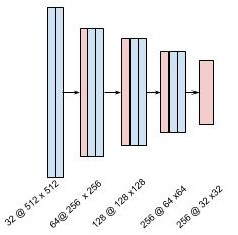
\includegraphics[scale=0.6]{Images/conv_enc}
  \caption[\textgreek{Στάδιο Κωδικοποίησης}]{\textgreek{Στάδιο κωδικοποίησης των ΣΝΔ} \textgreek{επίπεδο.}}
 \label{fig:encode_stage}
\end{figure}

\textgreek{Η εικόνα }\ref{fig:maxpool} \textgreek{μας δείχνει ένα παράδειγμα εφαρμογής ενός πυρήνα $3\times3$ πάνω σε ένα επίπεδο χαρακτηριστικών $5\times5$ εφαρμόζοντας την μέθοδο της μέγιστης συγκέντρωσης. Όπως βλέπουμε συγκεντρώνουμε το μέγιστο στοιχείο από τον $3\times3$ πυρήνα που ολισθαίνει σε όλο το επίπεδο ενός χάρτη χαρακτηριστικών, από αριστερά προς τα δεξιά.}

\begin{figure}[H]
 \centering
 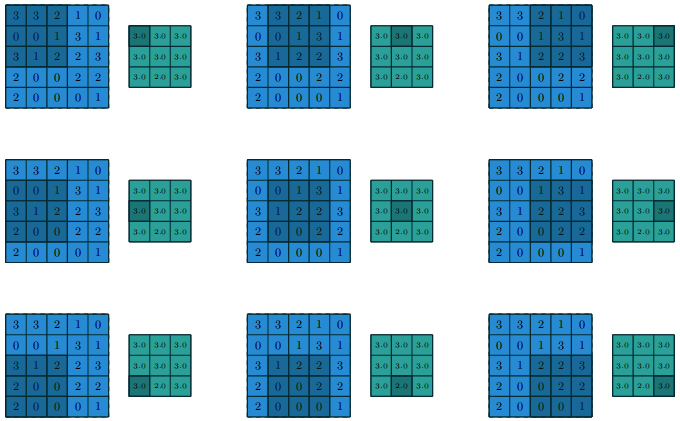
\includegraphics[scale=0.5]{Images/maxpool}
  \caption[\textgreek{Παράδειγμα Μέγιστη Συγκέντρωσης}]{\textgreek{Παράδειγμα της μεθόδου της μέγιστης συγκέντρωσης, εφαρμόζοντας ένα παράθυρο $3\times3$ σε ένα επίπεδο χαρακτηριστικών εισόδου $5\times5$ με μονό βήμα ολίσθησης. Τα βήματα είναι από αριστερά προς τα δεξιά} \cite{conv_arithmetic}.}
 \label{fig:maxpool}
\end{figure}

\subsection{\textgreek{Μονάδα Παράλληλης Επεξεργασίας Χαρακτηριστικών}}
\textgreek{Η παράλληλη μονάδα επεξεργασίας χαρακτηριστικών αποτελείται από 5 διαφορετικά τμήματα τα οποία δέχονται ως είσοδο τον χάρτη με τα κωδικοποιημένα χαρακτηριστικά από το στάδιο της κωδικοποίησης. Η εξίσωση }\ref{eqn:dilated_conv} \textgreek{μας δείχνει την συνέλιξη σε ένα επίπεδο σήμα εισάγοντας την διαστολή που υποδεικνύεται με $r$}.\textgreek{ Η συγκεκριμένη συνάρτηση υπάγεται στην θεωρία ως Διεσταλμένη Συνέλιξη} (Dilated Convolution) \textgreek{ενώ η εικόνα }\ref{fig:conv_ar_1} \textgreek{ μας δίνει μια διαίσθηση γύρω από αυτή την τεχνική.}

\begin{equation}
  \label{eqn:dilated_conv}
  g[i,j] = \sum_{k}\sum_{k} f[i+r\cdot k, j+r\cdot k]h[k,k] 
\end{equation}

\par
\textgreek{Πιο συγκεκριμένα, κάθε παρακλάδι της μονάδας επεξεργασίας διαφέρει στην διαστολή των στοιχείων του πυρήνα που αλληλεπιδρούν με την είσοδο (εικόνα }\ref{fig:parallel_unit}). \textgreek{Σκοπός αυτού του τμήματος είναι η μάθηση χαρακτηριστικών από διαφορετικά πεδία όρασης. Κάθε παρακλάδι διαθέτει έναν πυρήνα με διαφορετική διαστολή στο πρώτο επίπεδο. Ο πυρήνας σε όλους τους κλάδους έχει μέγεθος $3\times 3$, εκτός από το τελευταίο επίπεδο πριν την ένωση των χαρακτηριστικών όπου η πυρήνας έχει μέγεθος $1\times 1$. Στην εικόνα }\ref{fig:parallel_unit} \textgreek{βλέπουμε σε κάθε επίπεδο το μέγεθος κάθε επιπέδου και τον αριθμό του βάθους των φίλτρων τα οποία είναι 256, 128 και 128 αντίστοιχα. Ο λόγος που μειώνουμε τις διαστάσεις είναι για την μείωση των παραμέτρων κατά την εκπαίδευση. Επίσης, για να κρατήσουμε σταθερό το μέγεθος των χαρακτηριστικών και για να μην υπάρχει περαιτέρω αλλοίωση της πληροφορίας γεμίζουμε περιφερειακά με μηδενικά την είσοδο πριν την διαδικασία της συνέλιξης. Στο στάδιο της ένωσης πραγματοποιείται η πράξη της πρόσθεσης όλως των χαρακτηριστικών που καταλήγουν από κάθε κλάδο αντίστοιχα.}

\begin{figure}[H]
 \centering
 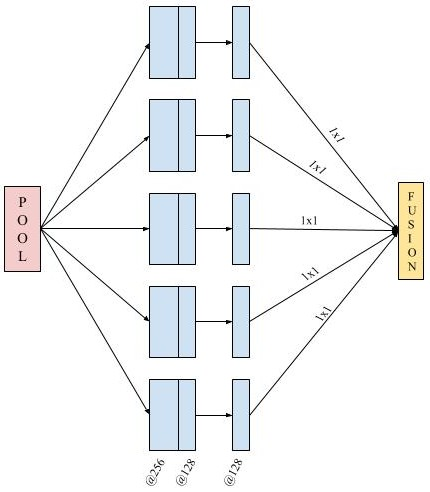
\includegraphics[scale=0.55]{Images/parallel_1}
  \caption[\textgreek{Παράλληλη Μονάδα Επεξεργασίας}]{\textgreek{Η παράλληλη μονάδα επεξεργασίας με τα 5 ξεχωριστά μονοπάτια. Το κάθε μονοπάτι έχει στο πρώτο επίπεδο συνέλιξης μια διαστολή: $3\times 3$, $6\times6$, $9\times9$, $12\times12$ και $1\times1$ αντίστοιχα. Επίσης, βλέπουμε και τον αριθμό των φίλτρων του κάθε επιπέδου συνέλιξης.} }
 \label{fig:parallel_unit}
\end{figure}


\textgreek{Παρακάτω βλέπουμε ένα παράδειγμα για την διεσταλμένη συνέλιξη όπου εφαρμόζουμε έναν πυρήνα $3\times3$ πάνω σε ένα επίπεδο εισόδου $7\times7$ με ολίσθηση του πυρήνα ίσο με 1 και χωρίς γέμισμα περιφερειακά της εισόδου με μηδενικά. Στην δική μας περίπτωση υπάρχει γέμισμα του χάρτη χαρακτηριστικών περιφερειακά με μηδενικά καθώς θέλουμε να κρατήσουμε το μέγεθος αναλλοίωτο αλλά και να προσπαθήσουμε να κρατήσουμε την θέση της πληροφορίας όσο περισσότερο γίνεται. 

\parΗ διεσταλμένη συνέλιξη γεμίζει τον πυρήνα του φίλτρου με μηδενικά ανάμεσα στα στοιχεία του πυρήνα. Για την ακρίβεια, για έναν ρυθμό διαστολής $\mathit{d}$ εισάγουμε $\mathit{d-1}$ μηδενικά ανάμεσα στα στοιχεία του πυρήνα και προφανώς για $d=1$ αναφερόμαστε σε μια τυπική συνέλιξη. Η συνέλιξη με διαστολή συνήθως χρησιμοποιείται για την αύξηση του δεκτικού πεδίου ενός νευρώνα χωρίς να χρειαστεί να αυξηθεί το μέγεθος του πυρήνα. Μία σημαντική ιδιότητα αυτής της τεχνικής είναι ο αριθμός των παραμέτρων ο οποίος αυξάνεται γραμμικά ενώ ο αριθμός του δεκτικού πεδίου αυξάνεται εκθετικά.}

\begin{figure}[H]
 \centering
 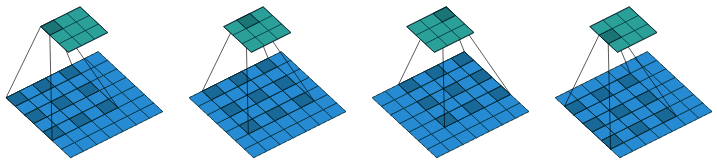
\includegraphics[scale=0.4]{Images/conv_ar_1}
 \caption[\textgreek{Διεσταλμένη Συνέλιξη}]{\textgreek{Συνέλιξη ενός πυρήνα μεγέθους $3\times3$ πάνω σε ένα επίπεδο εισόδου μεγέθους $7\times7$ και με διαστολή μεγέθους 2. Τα μπλε σκούρα στοιχεία δείχνουν την συμμετοχή για τον υπολογισμό της τιμής του στοιχείου (πράσινο σκούρο)} \cite{conv_arithmetic}. }
 \label{fig:conv_ar_1}
\end{figure}

\subsection{\textgreek{Στάδια Αποκωδικοποίησης}}
\subsubsection{\textgreek{Επισκόπηση}}
\textgreek{Παρακάτω θα εξηγήσουμε τις 2 παραλλαγές των μονάδων αποκωδικοποίησης που υλοποιήσαμε για να πειραματιστούμε με αυτές και να συγκρίνουμε τα αποτελέσματα τους στο πρόβλημα της Σημασιολογικής Κατάτμησης. Η κύρια διαφορά μεταξύ των 2 μονάδων είναι ο τρόπος που γίνεται η υπερδειγματοληψία. Η πρώτη μονάδα χρησιμοποιεί την μέθοδο της αποσυνέλιξης με εισαγωγή ενός βήματος για την επίτευξη της υπερδειγματοληψίας, ενώ στην δεύτερη μονάδα υλοποιήθηκε ένα επίπεδο διγραμμικής παρεμβολής που λειτουργεί με τον τρόπο που εξηγήσαμε στο τμήμα }\ref{sec:bilinear}.

\subsubsection{\textgreek{Μονάδα Αποσυνέλιξης Με Άλμα Ολίσθησης}}
\label{sec:sd-decoder}
\textgreek{Η συγκεκριμένη μονάδα αποκωδικοποίησης αποσκοπεί στην ανακατασκευή των χαρακτηριστικών από τον χάρτη χαρακτηριστικών πίσω στην μορφή της εικόνας. Η εικόνα }\ref{fig:deconv_1_stage} \textgreek{μας δείχνει την αρχιτεκτονική της μονάδας αποκωδικοποίησης. }

\begin{figure}[H]
 \centering
 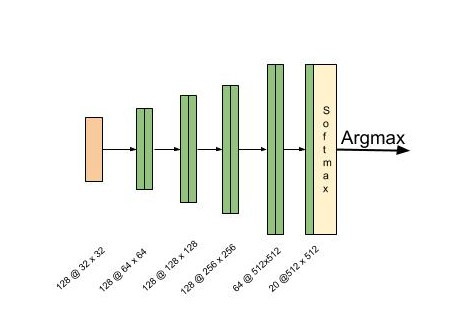
\includegraphics[scale=0.6]{Images/deconv_decoding}
  \caption[\textgreek{Στάδιο Αποκωδικοποίησης με βηματισμό}]{\textgreek{Στάδιο αποκωδικοποίησης του ΣΝΔ με χρήση επιπέδων αποσυνέλιξης.} }
 \label{fig:deconv_1_stage}
\end{figure}

\textgreek{Για να μπορέσουμε να εξηγήσουμε καλύτερα την μονάδα αποκωδικοποίησης θα πρέπει πρώτα να μιλήσουμε για την διαδικασία της αποσυνέλιξης ή ανάστροφης συνέλιξης όπως την βρίσκουμε στην βιβλιογραφία. Η ιδέα και η ανάγκη της ανάστροφης συνέλιξης προκύπτει από την επιθυμία να χρησιμοποιηθεί ένας μετασχηματισμός που να μας οδηγεί από τον χάρτη τον χαρακτηριστικών, δηλαδή στον μετασχηματισμό από ένα σχήμα κάποιου αντικειμένου πίσω στον ανασχηματισμό του σε σχέση με την εικόνα εισόδου. Με λίγα λόγια γίνεται μια ανακατασκευή της εικόνας από τα μεγάλων διαστάσεων χαρακτηριστικά. \par
Η τεχνική της ανάστροφης συνέλιξης μας οδηγεί από έναν χάρτη χαρακτηριστικών μικρού μεγέθους σε έναν χάρτη μεγαλύτερου μεγέθους ενώ συγκρατεί τα μοτίβα διασύνδεσης μεταξύ των νευρώνων. Η ανάστροφη συνέλιξη δουλεύει εναλλάσσοντας το μπροστινό πέρασμα με το πέρασμα της οπισθοδρόμησης της συνέλιξης. Με λίγα λόγια, η κανονική συνέλιξη με την ανάστροφη συνέλιξη είναι ο τρόπος με τον οποίο υπολογίζονται τα προς τα εμπρός και προς τα πίσω περάσματα }(feed-forward and backward passes). \par
\textgreek{Για παράδειγμα μπορεί ένας πυρήνας $\mathbf{w}$ να ορίζει μια συνέλιξη όπου τα περάσματα (εμπρός-πίσω) να υπολογίζονται από έναν πίνακα $\mathbf{C}$ και $\mathbf{C}^{T}$ αντίστοιχα, αλλά επίσης αν αναστρέψουμε τους πίνακες ορίζουμε την ανάστροφη συνέλιξη ορίζοντας τους πίνακες ως $\mathbf{C}^{T}$ και $(\mathbf{C}^{T})^{T} = \mathbf{C}$ για τα εμπρός και πίσω περάσματα αντίστοιχα. Τέλος, το τελευταίο επίπεδο πριν την εφαρμογή του επιπέδου} softmax \textgreek{έχουμε ένα επίπεδο με αριθμό βάθους χαρτών ίσο με 20, όσο είναι και οι κατηγορίες αντικειμένων. Κάθε επίπεδο του βάθους από τα 20 επίπεδα αποτελεί ένα }heatmap \textgreek{της κάθε κλάσης ως προς τις υπόλοιπες. Εφαρμόζοντας την }softmax \textgreek{μετασχηματίζεται η έξοδος σε μια κατανομή πιθανοτήτων. }   

\subsubsection{\textgreek{Διγραμμική Μονάδα Αποκωδικοποίησης}}

\textgreek{Η διγραμμική μονάδα αποκωδικοποίησης όπως βλέπουμε στην εικόνα }\ref{fig:bilinear_deconv} \textgreek{έχει πανομοιότυπη αρχιτεκτονική με την προηγούμενη μονάδα }\ref{sec:sd-decoder}, \textgreek{με την διαφορά στην μέθοδο που επιτυγχάνεται η υπερδειγματοληψία. Για την υπερδειγματοληψία του χάρτη χαρακτηριστικών χρησιμοποιείται η μέθοδος της διγραμμικής παρεμβολής. Κατά την διγραμμική παρεμβολή, ένα στοιχείο δημιουργείται από μια σταθμισμένη μέση τιμή από τέσσερα γειτονικά στοιχεία από τον χάρτη χαρακτηριστικών εισόδου. Το επίπεδο αυτό δεν διαθέτει παραμέτρους μάθησης. }

\begin{figure}[H]
 \centering
 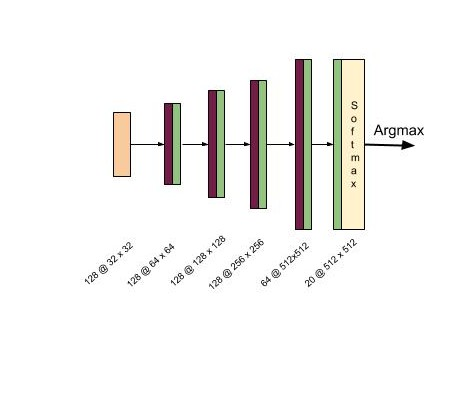
\includegraphics[scale=0.6]{Images/bilinear_conv}
  \caption[\textgreek{Διγραμμική Μονάδα Αποκωδικοποίησης}]{\textgreek{Στάδιο αποκωδικοποίησης του ΣΝΔ με χρήση επιπέδων διγραμμικής παρεμβολής για την υπερδειγματοληψία των χαρακτηριστικών. Τα μωβ επίπεδα υποδεικνύουν το επίπεδο της διγραμμικής παρεμβολής.}}
 \label{fig:bilinear_deconv}
\end{figure}
\pagebreak
\subsection{\textgreek{Ολοκληρωμένες Αρχιτεκτονικές}}
\textgreek{Η εικόνα }\ref{fig:systems} \textgreek{μας δείχνει τις μονάδες των αρχιτεκτονικών που περιγράψαμε προηγουμένως  μαζί με τις μονάδες μετά-επεξεργασίας που θα αναλύσουμε στο επόμενο κεφάλαιο. }

\begin{figure}[h]
\centering

\begin{subfigure}[b]{1\linewidth}
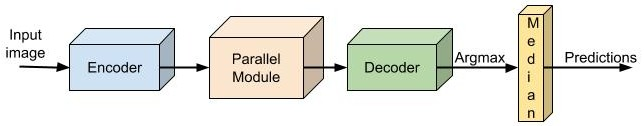
\includegraphics[scale=0.6]{Images/whole_arch_1}
 \caption{\textgreek{Ολοκληρωμένη αρχιτεκτονική με την μονάδα μετα-επεξεργασίας Μεσαίου Φίλτρου.}}
 \end{subfigure}
 \\[1cm]
 \begin{subfigure}[b]{1\linewidth}
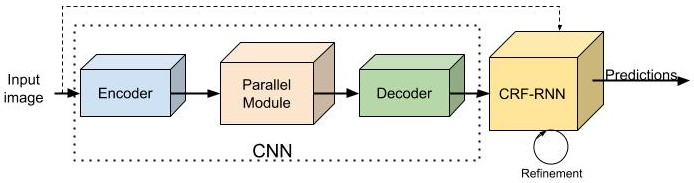
\includegraphics[scale=0.6]{Images/whole_arch_2}
\caption{\textgreek{Ολοκληρωμένη αρχιτεκτονική με την μονάδα μετα-επεξεργασίας ΤΥΣΠ-ΕΝΔ.}}
\end{subfigure}

\caption[\textgreek{Αρχιτεκτονικές ΣΝΔ}]{\textgreek{Ολοκληρωμένες Αρχιτεκτονικές.}}
\label{fig:systems}
\end{figure}


